Eine radioaktive Quelle (Am241) wird als $\alpha$-Strahler verwendet. Die emittierten Teilchen werden durch Blenden
kollimiert, sodass sie auf parallelen Bahnen zueinander auf eine dünne Goldfolie treffen. Es wird eine Folie aus Gold
gewählt, da sich dieses Element einfach zu einer dünnen Schicht verarbeiten lässt und eine hohe Atommasse besitzt, sodass
viele Wechselwirkungen stattfinden können.

An der Folie werden die Teilchen
in verschiedene Richtungen bzw. unter verschiedenen Winkeln gestreut, was mit einem Surface-Barrier-Detektor vermessen
werden kann. Der Detektor und ein Verstärker verstärken die aufgenommenen Impulse, die durch auftreffende Teilchen erzeugt
werden. Mit einem Oszilloskop kann eine Energieverlustmessung durchgeführt werden. Des Weiteren steht ein Zähler zur
Verfügung, mit dem Messungen zur Bestimmung des Streuquerschnitts durchgeführt werden können.

Der Aufbau befindet sich in einem Vakuumbehälter, da in diesem Versuch die $\alpha$-Strahlung in Luft lediglich eine
Reichweite von etwa 1,5cm hat.

\begin{figure}
\centering
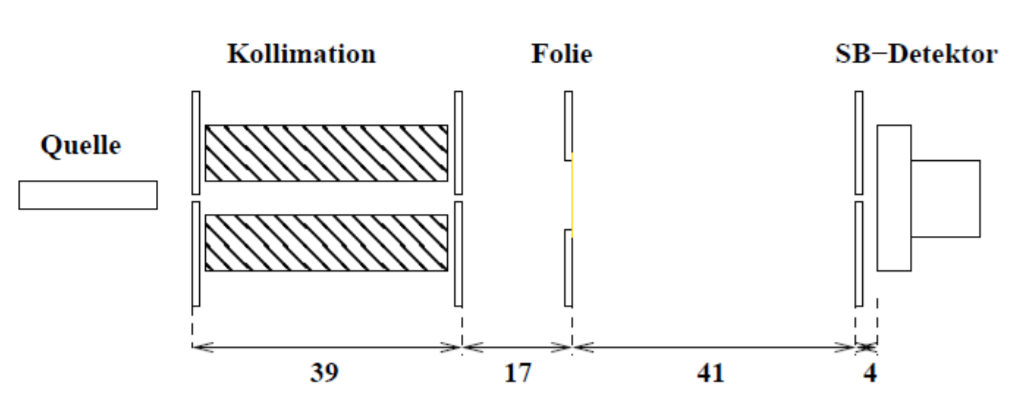
\includegraphics[width=\textwidth]{aufbau.png}
\caption{Schematische Darstellung der Messapparatur \cite[2]{anleitung}.}
\label{fig:aufbau}
\end{figure}
